\section{Predecir si los alumnos van a aprobar}

Hemos estudiado alguno de los factores que afectan a la nota final de los alumnos de matemáticas, a continuación utilizaremos estas métricas para poder estimar la probabilidad de que un alumno apruebe.

Para ello construiremos un modelo LOGIT, el cual se basa en la regresión lineal múltiple y en la función sigmoide para dar una predicción de la calificación de un estudiante.

En nuestro caso la variable endógena o explicada será la nota final de los alumnos, y las variables exógenas o explicativas los factores que hemos estudiado anteriormente. La perturbación $u$ recoge todos los factores que afectan a la nota final y que no están incluidas en el modelo (como por ejemplo la relación del alumno con su familia).
\begin{equation*}
        z = \beta_{1} + \beta_{2}\text{faltas} + \beta_{3}\text{internet} + \beta_{4} \text{clases particulares} + \beta_{5}\text{alcohol} + u
\end{equation*}

Los parámetros $\beta_{i}$ miden el impacto de las variables explicativas en la variables endógena, y al ser cantidades desconocidas trataremos de estimarlas mediante el entrenamiento del modelo. El parámetro $\beta_{1}$ es el termino independiente el cual aun siendo imprescindible en el modelo no interpretaremos.

El modelo LOGIT estima la probabilidad de naturaleza dictotómica, en nuestro caso aprobar $y=1$ o suspender $y=0$.
\begin{equation*}
    \text{probabilidad aprobar} \equiv P(y = 1) = \frac{e^{z}}{1 + e^{z}} 
\end{equation*}

Una vez entrenado el modelo en python obtenemos el siguiente resumen del modelo.
\begin{figure}[H]
    \begin{center}
        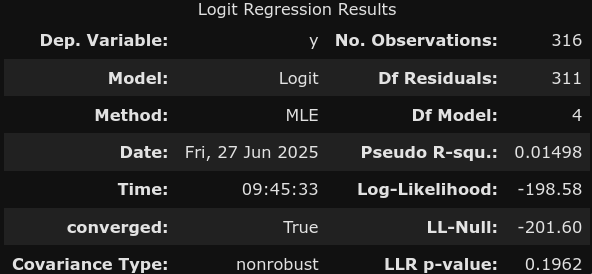
\includegraphics[width=0.95\textwidth]{figures/logit-summary.png}
    \end{center}
    \caption{Resumen del modelo LOGIT.}\label{fig:logit-summary}
\end{figure}

Lo más destacado de este resumen es el \textit{Log-Likelihood} que al ser bajo ($-198$) da indicios de que el modelo es bueno.

El resumen también ofrece información de los parámetros $\beta_{i}$ del modelo. En concreto, realiza un contraste de hipótesis para determinar si el parámetro aporta información relevante al modelo.

\begin{figure}[H]
    \begin{center}
        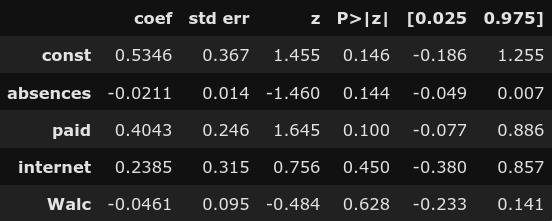
\includegraphics[width=0.95\textwidth]{figures/parameters.png}
    \end{center}
    \caption{Información de los parámetros.}\label{fig:}
\end{figure}

En nuestro caso vemos que las variables exógenas que hemos elegido no son las mejores ya que ninguna sería considerada como relevante, sin embargo las más significativas son el número de asistencias en clase y si el alumno asiste a clases particulares.

Aun con todo, el modelo tiene una \textit{accuracy} del $69\%$.

\begin{figure}[H]
    \begin{center}
        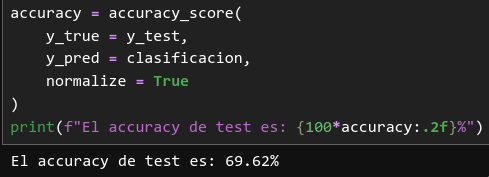
\includegraphics[width=0.95\textwidth]{figures/accuracy.png}
    \end{center}
    \caption{Accuracy del modelo LOGIT.}\label{fig:accuracy}
\end{figure}

Entonces, en nuestro modelo, un alumno que no asiste a clases particulares pero que no falta a clase (solo ha tenido 5 faltas), que toma mucho alcohol los fines de semana y que tiene acceso a internet tendría una probabilidad de aprobar del $60\%$.

\begin{figure}[H]
    \begin{center}
        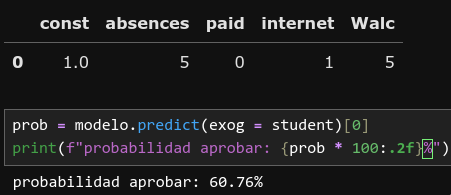
\includegraphics[width=0.95\textwidth]{figures/prob-aprobar-1.png}
    \end{center}
    \caption{Probabilidad de aprobar del alumno.}\label{fig:prob-aprobar-1}
\end{figure}

Si ese mismo alumno hubiese faltado 20 veces a clase, ahora su probabilidad de aprobar sería del $53\%$.
\begin{figure}[H]
    \begin{center}
        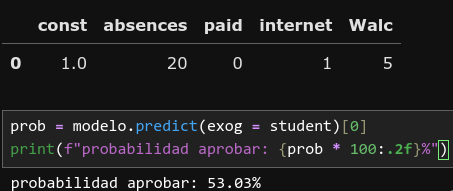
\includegraphics[width=0.95\textwidth]{figures/prob-aprobar-2.png}
    \end{center}
    \caption{Probabilidad de aprobar del alumno si faltase a 20 clases.}\label{fig:prob-aprobar-2}
\end{figure}

Por último, si el alumno original hubiese tomado clases particulares durante el curso, tendría una probabilidad de aprobar del $69\%$.
\begin{figure}[H]
    \begin{center}
        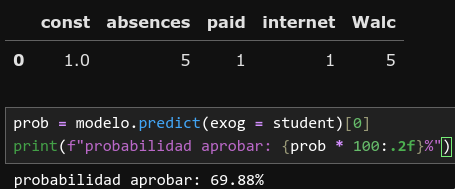
\includegraphics[width=0.95\textwidth]{figures/prob-aprobar-3.png}
    \end{center}
    \caption{Probabilidad de aprobar del alumno si tomase clases particulares.}\label{fig:prob-aprobar-3}
\end{figure}
